\documentclass[11pt,letterpaper]{article}

\usepackage[margin=1in]{geometry}
\usepackage{tikz}
\usepackage{xcolor}
\usepackage{hyperref}
\usepackage{booktabs}
\usepackage{tabularx}
\usepackage{enumitem}
\usepackage{fancyhdr}
\usepackage{graphicx}
\usepackage{float}
\usepackage{caption}
\usepackage{amsmath}
\usepackage{fontenc}

\usetikzlibrary{shapes.geometric, arrows.meta, positioning, fit, backgrounds, calc, shadows}

\definecolor{noaablue}{HTML}{003087}
\definecolor{noaalight}{HTML}{4A90D9}
\definecolor{awsorange}{HTML}{FF9900}
\definecolor{vpcgreen}{HTML}{1B660F}
\definecolor{securityred}{HTML}{CC2936}
\definecolor{neptunepurple}{HTML}{6B48FF}
\definecolor{agentcoregold}{HTML}{D4A017}
\definecolor{lightgray}{HTML}{F5F5F5}

\pagestyle{fancy}
\fancyhf{}
\fancyhead[L]{\small\textcolor{noaablue}{NOAA/NWS/NCEP/EMC --- CAT Unit}}
\fancyhead[R]{\small\textcolor{noaablue}{Multi-Pillar MCP for OMD}}
\fancyfoot[C]{\thepage}
\renewcommand{\headrulewidth}{0.4pt}

\hypersetup{colorlinks=true, linkcolor=noaablue, urlcolor=noaalight}

\title{%
    \vspace{-1cm}
    \textcolor{noaablue}{\Large\textbf{From Monolith to Multi-Pillar:}}\\[0.2cm]
    \textcolor{noaablue}{\Large\textbf{Scaling MCP/RAG Code Intelligence Across the OMD Portfolio}}\\[0.3cm]
    \large A Six-Month Retrospective and the Architectural Inflection Point\\[0.2cm]
    \normalsize NOAA Office of Modeling Development --- Configuration Management Discovery Year~1
}
\author{%
    Terry McGuinness\\
    \small Computing \& Advanced Technologies (CAT) Unit\\
    \small Environmental Modeling Center, NCEP/NWS/NOAA\\
    \small \texttt{terry.mcguinness@noaa.gov}
}
\date{May 22, 2026}

\begin{document}
\maketitle
\thispagestyle{fancy}

\begin{abstract}
\noindent
Over six months we built, deployed, and validated a 52-tool MCP/RAG
server (\texttt{agentcore-mcp-rag}) that puts AI-assisted code
intelligence on top of NOAA's Global Forecast System workflow. The
system ingests $\sim$149\,000 graph nodes (Neptune) and $\sim$199\,000
documents (OpenSearch) drawn from the \texttt{develop} branch of
\texttt{NOAA-EMC/global-workflow} and the surrounding ecosystem
(EE2 standards, J-Job documentation, ingested community summaries,
external documentation crawls). The server is deployed as an AWS
Bedrock AgentCore Runtime and accessed by developers through a
CAC-authenticated bastion path from their GFE laptops. Every objective
on the original deployment scorecard has been met: HEALTHY 4/4 on every
component, 7/9 on the per-tool functional smoke suite, sub-200~ms
latency on representative queries, and live 100\% similarity on
domain-specific searches such as MPAS Voronoi mesh content that we
explicitly rebuilt from a path-prefix crawler bug last week.

This paper argues that hitting that scorecard is not the end of the
story --- it is the moment the next-level architectural problem
becomes visible. The deep dive on \texttt{dev/sfs} (the freshly
connected Seasonal Forecast System branch) revealed that
\texttt{NOAA-EMC/global-workflow.git} is not one system but
\textbf{six}: \texttt{develop} plus five active \texttt{dev/*} pillars
(\texttt{dev/gfs.v17}, \texttt{dev/gfs.v16}, \texttt{dev/gcafs.v1},
\texttt{dev/jedi-gfs}, \texttt{dev/sfs}), each representing a distinct
intellectual program with its own user community, divergence trajectory,
and lifecycle. The current monolithic ingestion of \texttt{develop} is
silently misleading users working on the other five pillars.

We present the multi-pillar architecture that resolves this --- a
catalog-driven tenant model with branch-scoped data isolation, content-
addressed dedupe, shared-component inheritance, and lifecycle-aware
attribution --- and we identify \texttt{dev/sfs} as the natural pilot
target. The paper is structured as a one-stop briefing for OMD
management: the journey, the inflection point, the architecture, the
risk-managed rollout, and the one-week-actionable next step.
\end{abstract}

\section{The Six-Month Journey}

\subsection{Where we started (December 2025)}

The original premise was straightforward: take the GFS workflow code,
build a Neo4j graph from the AST + import + invocation relationships,
build a ChromaDB vector store from the documentation and code-with-
context corpora, and expose a Model Context Protocol (MCP) server with
tools for code analysis, semantic search, EE2 compliance checks, and
operational guidance. A developer using the Kiro IDE would get
GraphRAG-quality answers about j-jobs, ex-scripts, ush helpers, and
parm configurations without leaving their editor.

Phase 48 ported that vision to AWS-native services. Neo4j became
Neptune. ChromaDB became OpenSearch. Sentence-Transformers
\texttt{all-mpnet-base-v2} became Bedrock Titan Embed Text v2 at 1024
dimensions. The Node.js runtime (still in production for backward
compatibility) became a Python port that runs as an ARM64 container on
Bedrock AgentCore Runtime. Every piece of the data plane lives inside
a private VPC; there is no internet-facing service surface. CAC/PIV
authentication carries the identity from the GFE laptop, through an
NIH bastion, into the EC2 development host, and through to AgentCore
via IAM SigV4.

\subsection{Where we are (May 22, 2026)}

The system that exists today:

\begin{itemize}[leftmargin=*]
    \item \textbf{52 tools across 9 modules}: workflow info, code
    analysis, semantic search, EE2 compliance, operational guidance,
    GraphRAG, GitHub integration, SDD workflow tracking, and built-in
    utilities.
    \item \textbf{Data plane}: Neptune (148\,976 nodes, 2.82M
    relationships) + OpenSearch (15 indices, 198\,832 documents
    spanning the workflow itself, J-Job headers, code-with-context,
    EE2 standards, and community summaries).
    \item \textbf{Live AgentCore Runtime}:
    \texttt{mdc\_mcp\_rag\_server\_python-v5K2F8BGrN}, version 16,
    image \texttt{python-titan-v5}, status READY.
    \item \textbf{Health}: HEALTHY 4/4 on the synthetic check; 7/9 pass
    on the new functional smoke suite (with two known fails being
    pre-existing container-state gaps now under remediation).
\end{itemize}

\subsection{The week-of-arrival path}

The last six weeks alone delivered: Phase~C-3 Bedrock IAM enablement;
the Python cutover (now the active MCP target); Bedrock-native
embedding swap to Titan~1024; manifest gap closure (12~pending URL
sources, including newly added MPAS, CATChem, CECE, CDEPS, Land-DA,
uwtools, UFS-SRW, GSI, HAFS); the MPAS path-prefix crawler bugfix
that turned \texttt{doc\_count: 0} into \texttt{doc\_count: 439}
real Voronoi-mesh documents; functional smoke tests that catch
``tool registered but data layer broken'' silently-passing failures;
governance changes that prevent recurrence (Spec-First gate, git
operation policy, edit-time hooks); and an end-to-end CAC connectivity
diagram that lets a new developer land on the system in two hours.

The story is not "we are done." The story is "we did exactly what we
set out to do, and the act of doing it surfaced the next problem."

\section{The Inflection Point: \texttt{dev/sfs} Forces the Multi-Pillar Question}

\subsection{What the deep dive showed}

On May~22, 2026 a new submodule \texttt{global-workflow\_dev-sfs} was
added to track the Seasonal Forecast System branch. We performed a
deep dive on it, expecting an incremental feature branch.
What we found, summarized in Table~\ref{tab:pillars}, is that the
\texttt{NOAA-EMC/global-workflow.git} repository hosts \emph{six
living trajectories} that all share the same parent commit history
but have meaningfully different code, intent, user communities, and
lifecycle states.

\begin{table}[H]
\centering
\caption{The six development pillars inside one repository (state on 2026-05-22)}
\label{tab:pillars}
\small
\begin{tabularx}{\textwidth}{lXrrr}
\toprule
\textbf{Pillar} & \textbf{Purpose} & \textbf{Ahead} & \textbf{Behind} & \textbf{Diff (files)} \\
\midrule
\texttt{develop} & Canonical operational baseline & --- & --- & --- \\
\texttt{dev/gfs.v17} & Next-generation coupled GFS (operational target) & 71 & 163 & 894 \\
\texttt{dev/gfs.v16} & Current operational v16 (parallel evolution) & 855 & 2\,053 & 2\,287 \\
\texttt{dev/gcafs.v1} & Global Chemistry \& Aerosol Forecast v1 & 33 & 115 & 667 \\
\texttt{dev/jedi-gfs} & JEDI-based DA experimentation (5\,mo stale) & 0 & 179 & 834 \\
\texttt{dev/sfs} & S2S post-processing pipeline (new --- in PR review) & 284 & 0 & 112 \\
\bottomrule
\end{tabularx}
\end{table}

The \texttt{dev/sfs} branch alone adds three new J-Jobs
(\texttt{JGLOBAL\_ATMOS\_POST}, \texttt{\_OCN\_POST}, \texttt{\_ICE\_POST}),
six new ush helpers (\texttt{process\_atmos\_\{6hrly,daily\}.sh},
\texttt{process\_ocean\_\{6hrly,daily,monthly\}.sh}), three Python
ocean-diagnostics scripts implementing CPC operational products
(Ocean Heat Content, Tropical Cyclone Heat Potential, depth of 20\,$^\circ$C
isotherm), 20 Jinja archive templates parameterized per ensemble
member, 11 CI test cases, 7 platform module files, and the workflow
generator integration to wire it all into the Rocoto task graph.

None of these artifacts exist on \texttt{develop}.

\subsection{The configuration-management hazard, made concrete}

A user working on \texttt{dev/sfs} who asks the AgentCore MCP
``what are the inputs to \texttt{JGLOBAL\_ATMOS\_POST}?'' receives,
today, the answer: ``not found.'' That is not the worst case --- it is
loud and the user knows to look elsewhere.

The worst case is when a file \emph{exists on both branches with
divergent behaviour}. A user working on \texttt{dev/gfs.v17} who asks
``what does the forecast driver do?'' receives a develop-branch
answer that is silently wrong. The 894-file divergence guarantees this
class of false-positive will grow as v17 development progresses. The
question is not \emph{whether} this is a problem --- it is, today, on
develop alone --- but \emph{how soon} the operational community
notices that the AI assistant is feeding them stale information.

\subsection{Why this is the right time to address it}

Three properties of the current moment make this the architecturally
right time to act:

\begin{enumerate}[leftmargin=*]
    \item \textbf{The single-tenant system is healthy and proven.}
    Six months of investment has produced a working baseline.
    Multi-tenancy can be added \emph{on top of} a working system
    rather than retrofit into a struggling one.
    \item \textbf{The smallest possible pilot is available.}
    \texttt{dev/sfs} (112 files / +3\,829 lines, fully synced with
    develop today) is the cheapest possible target on which to
    validate the approach before scaling to \texttt{dev/gfs.v17}
    (where the operational stakes are highest).
    \item \textbf{The governance to prevent silent regressions
    is now in place.} The Spec-First gate, the functional smoke
    suite, the git operation policy, and the file-edit hooks were
    all built in the last two weeks specifically to catch the kind
    of "everything passes but the data layer is wrong" failure that
    multi-tenancy makes more probable.
\end{enumerate}

\section{The Multi-Pillar Architecture}

\subsection{Core principle: same image, different data view}

Figure~\ref{fig:topology} shows the proposed topology. Every tenant
runs the \emph{same} Docker image. The 52-tool surface is identical;
the tools have no idea which tenant they are answering for. What
differs between tenants is:

\begin{itemize}[leftmargin=*]
    \item The OpenSearch index prefix (e.g.\
    \texttt{gw\_sfs\_workflow\_docs} vs \texttt{gw\_workflow\_docs}).
    \item The Neptune label prefix (e.g.\ \texttt{GW\_SFS\_File} vs
    \texttt{GW\_File}) since AWS Neptune does not have multi-database
    semantics.
    \item The \texttt{WORKFLOW\_REF} environment variable (e.g.\
    \texttt{NOAA-EMC/global-workflow@dev/sfs} vs \texttt{...@develop}).
    \item The \texttt{tenant\_id} attached to every response for
    attribution.
\end{itemize}

\begin{figure}[H]
\centering
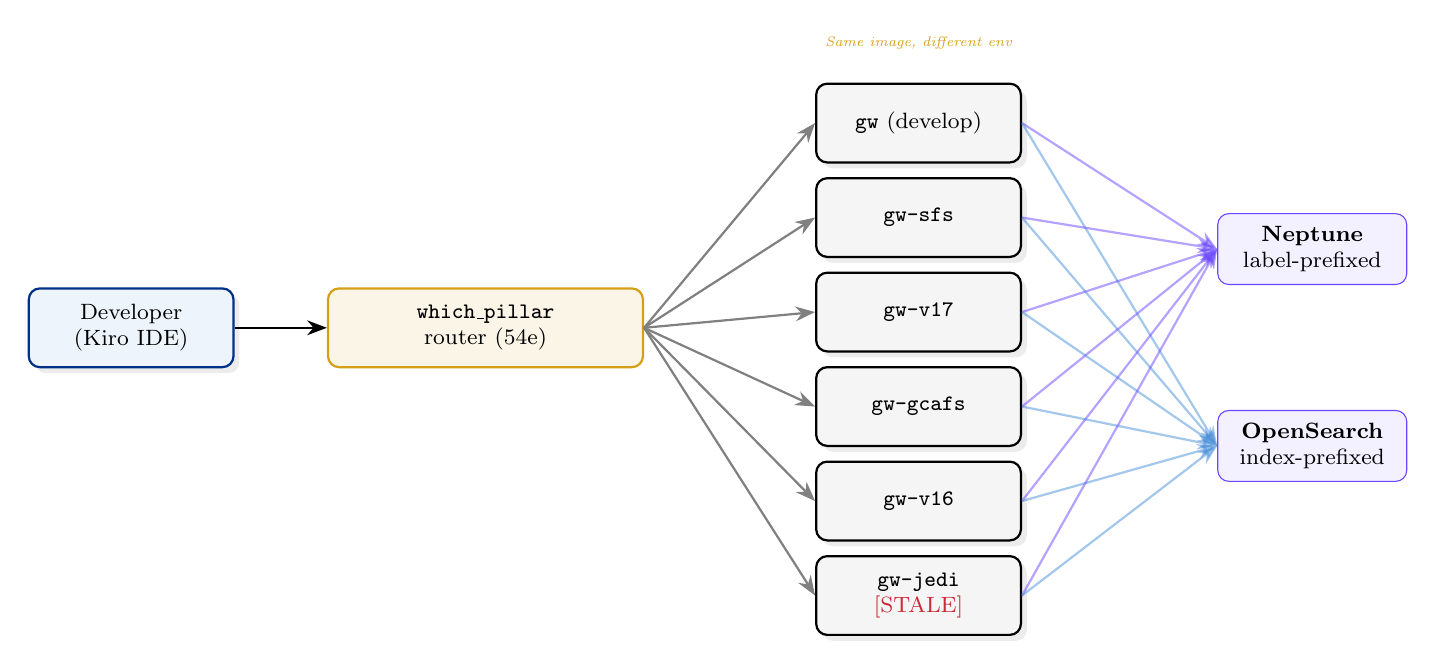
\begin{tikzpicture}[
    every node/.style={font=\footnotesize},
    pillar/.style={rectangle, draw, rounded corners=4pt, minimum width=2.6cm, minimum height=1cm, align=center, thick, drop shadow={opacity=0.15}},
    runtime/.style={rectangle, draw=agentcoregold, fill=agentcoregold!10, rounded corners=4pt, minimum width=4cm, minimum height=1cm, align=center, thick},
    data/.style={rectangle, draw=neptunepurple, fill=neptunepurple!8, rounded corners=4pt, minimum width=2.4cm, minimum height=0.9cm, align=center},
    arrow/.style={-{Stealth[length=2.5mm]}, thick}
]

% User
\node[pillar, fill=noaalight!10, draw=noaablue] (user) at (0, 0) {Developer\\(Kiro IDE)};

% Router
\node[runtime] (router) at (4.5, 0) {\texttt{which\_pillar}\\router (54e)};

% Six tenants
\node[pillar, fill=lightgray] (gw) at (10, 2.6) {\texttt{gw} (develop)};
\node[pillar, fill=lightgray] (gwsfs) at (10, 1.4) {\texttt{gw-sfs}};
\node[pillar, fill=lightgray] (gwv17) at (10, 0.2) {\texttt{gw-v17}};
\node[pillar, fill=lightgray] (gwgcafs) at (10, -1) {\texttt{gw-gcafs}};
\node[pillar, fill=lightgray] (gwv16) at (10, -2.2) {\texttt{gw-v16}};
\node[pillar, fill=lightgray] (gwjedi) at (10, -3.4) {\texttt{gw-jedi}\\\textcolor{securityred}{[STALE]}};

% Shared image label
\node[font=\tiny\itshape, text=agentcoregold, above=0.3cm of gw] (img) {Same image, different env};

% Data layer
\node[data] (neptune) at (15, 1) {\textbf{Neptune}\\label-prefixed};
\node[data] (os) at (15, -1.5) {\textbf{OpenSearch}\\index-prefixed};

% Arrows
\draw[arrow] (user.east) -- (router.west);
\foreach \t in {gw, gwsfs, gwv17, gwgcafs, gwv16, gwjedi} {
    \draw[arrow, gray] (router.east) -- (\t.west);
}
\foreach \t in {gw, gwsfs, gwv17, gwgcafs, gwv16, gwjedi} {
    \draw[arrow, neptunepurple, opacity=0.5] (\t.east) -- (neptune.west);
    \draw[arrow, noaalight, opacity=0.5] (\t.east) -- (os.west);
}

\end{tikzpicture}
\caption{Multi-pillar topology. One image, one router, $N$ tenants, one shared data plane with prefix-based scoping.}
\label{fig:topology}
\end{figure}

\subsection{Workstream decomposition}

\begin{table}[H]
\centering
\caption{The seven workstreams of the OMD Multi-Pillar Initiative}
\small
\begin{tabularx}{\textwidth}{llX}
\toprule
\textbf{ID} & \textbf{Workstream} & \textbf{What it delivers} \\
\midrule
54a & Tenant catalog schema & YAML schema: \texttt{tenant\_id}, repo, branch, \texttt{extends:}, lifecycle, staleness, secrets \\
54b & Per-tenant data isolation & OpenSearch index prefix + Neptune label prefix; 52 tools made tenant-aware \\
54c & Shared-component inheritance & \texttt{extends: [ufs]} with catalog-time vs query-time semantics decided \\
54d & Branch-scoped tenants + dedupe & Six \texttt{gw-*} tenants on the same image; SHA-keyed content dedupe (critical-path) \\
54e & Routing \& attribution & \texttt{which\_pillar} recommender; \texttt{tenant\_id} on every response \\
54f & Headless auth broker (parallel) & \texttt{age}/\texttt{sops} or Vault; arXiv + Semantic Scholar pilots \\
54g & Lifecycle \& staleness (NEW) & Auto-deprecation on branch merge; \texttt{[STALE]} marker at threshold \\
\bottomrule
\end{tabularx}
\end{table}

\subsection{Pilot rollout sequence}

The Initiative is decomposed into a risk-managed rollout that
validates the cheapest possible pilot before committing to the
operational prize:

\begin{enumerate}[leftmargin=*]
    \item \textbf{\texttt{omd-tenants-1-foundation}} (54a + 54b
    minimum). Existing AgentCore Runtime becomes a single tenant
    \texttt{gw}; nothing changes for users but plumbing is in place.
    \item \textbf{\texttt{omd-tenants-2-sfs-pilot}} (54d). Stand up
    \texttt{gw-sfs} against \texttt{dev/sfs}, ingest only the 112-file
    diff, run the branch-isolation probe, prove dedupe works.
    \item \textbf{\texttt{gw-v17-tenant}}. Repeat for \texttt{dev/gfs.v17}
    --- the operational prize. The v17 community starts getting
    AI-assisted code analysis that is correct.
    \item Remaining pillars (\texttt{gw-gcafs}, \texttt{gw-v16},
    \texttt{gw-jedi}) in order of community urgency.
    \item \texttt{extends:} (54c) + UFS tenant when 2+ pillars share UFS.
    \item Routing + lifecycle (54e + 54g) when 3+ tenants exist.
    \item Auth broker (54f) parallel to all of the above.
\end{enumerate}

\section{Cost \& Risk}

\subsection{Storage / cost projections}

Naive 6$\times$ ingestion would 6$\times$ the data plane cost.
Content-addressed dedupe (workstream 54d) is what makes the model
economically viable. The merge-base structure of the six pillars is
favourable: \texttt{dev/sfs} shares 99.6\% of files with develop;
\texttt{dev/gfs.v17} shares 90.5\%; \texttt{dev/gcafs.v1} shares 96\%.
Only the divergent slice needs new vectors and new graph nodes; the
rest is referenced from the develop tenant via SHA-keyed dedupe.

\begin{table}[H]
\centering
\caption{Approximate ingestion cost per pillar (with dedupe)}
\small
\begin{tabularx}{\textwidth}{lrXr}
\toprule
\textbf{Pillar} & \textbf{Diff size} & \textbf{Dedupe basis} & \textbf{Net new \$/month} \\
\midrule
\texttt{gw-sfs} & 112 files & vs develop (99.6\% shared) & $\sim$\$2 \\
\texttt{gw-v17} & 894 files & vs develop (90.5\% shared) & $\sim$\$15 \\
\texttt{gw-gcafs} & 667 files & vs develop (96\% shared) & $\sim$\$8 \\
\texttt{gw-v16} & 2287 files & vs develop (76\% shared) & $\sim$\$30 \\
\texttt{gw-jedi} & 834 files & vs develop & $\sim$\$12 \\
\midrule
\textbf{Total above develop baseline} & & & \textbf{$\sim$\$67/month} \\
\bottomrule
\end{tabularx}
\end{table}

This is small compared to the existing baseline (existing Neptune +
OpenSearch are sunk; the marginal Bedrock embedding cost is small).

\subsection{Top risks}

Three risks dominate the rollout:

\begin{enumerate}[leftmargin=*]
    \item \textbf{Content-addressed dedupe correctness (R3).} If
    dedupe is buggy, two tenants can return each other's data. This is
    the worst class of failure in a multi-tenant system. Mitigation: a
    dedicated parity probe in 54d that fires queries known to have
    different answers per tenant and asserts they do.
    \item \textbf{Tenant routing UX (R4).} If users have to learn six
    tenant names, adoption suffers. The \texttt{which\_pillar}
    recommender (54e) is on the critical path, not nice-to-have.
    \item \textbf{Per-tenant runtime cost vs routing complexity (R7).}
    One AgentCore Runtime per tenant is clean but expensive. One
    Runtime serving all tenants with header-based routing is cheap but
    adds a routing layer to operate. Decision: spike both in 54b.
\end{enumerate}

\section{What This Means for OMD Management}

\subsection{Six-month story arc, in one paragraph}

In December~2025 we set out to put AI-assisted code intelligence on
top of the Global Forecast System. By May~2026 we had a 52-tool
production-grade MCP/RAG server running on AWS Bedrock AgentCore,
serving CAC-authenticated developers, with $\sim$199K embedded
documents and $\sim$2.9M graph relationships. The act of finishing
that work surfaced the next problem: the OMD portfolio is not one
program but at least six (and growing), and the monolithic system
serves only one of them. The architecture to address that
\emph{(multi-pillar tenant model with branch-scoped data isolation
and lifecycle-aware attribution)} is well-understood, the pilot
target \emph{(\texttt{dev/sfs})} is the smallest possible validation
of the approach, and the engineering that prevents silent regressions
\emph{(spec-first gate, functional smoke tests, edit-time hooks)} is
already in place.

\subsection{Why this paper is the publication}

Six months of work culminate in an architectural inflection. The
publishable insight is not "we built an MCP server" --- many groups
have done that --- it is the journey from \emph{single-program
monolith} to \emph{recognition that scientific computing organizations
maintain portfolios of intellectually distinct development trajectories
that look like branches of one repository but are functionally
separate systems}. Configuration-management hazard, content-addressed
dedupe, tenant lifecycle, branch-isolation probes, and auto-deprecation
on merge are concepts that generalize beyond NOAA --- any organization
maintaining $N$ branches of one operational system has the same
problem.

\subsection{The one-week-actionable next step}

This paper accompanies the Phase~54 SDD Initiative
(\texttt{Phase-54-OMD-Multi-Program-MCP-Initiative} on the
\texttt{global-workflow.wiki}) and a companion Kiro spec
\texttt{omd-tenants-1-foundation} on \texttt{develop\_aws}. The
recommended first action: author and approve the spec for workstreams
54a + 54b, with \texttt{dev/sfs} as the validation target. The total
engineering effort to get from "spec approved" to "branch-isolation
probe passing on \texttt{gw-sfs}" is estimated at one engineering
sprint (two weeks).

\section{References \& Companion Artifacts}

\begin{itemize}[leftmargin=*]
    \item \textbf{Wiki Initiative}: \texttt{Phase-54-OMD-Multi-Program-MCP-Initiative.md} (refreshed 2026-05-22)
    \item \textbf{Connectivity diagram}: \texttt{docs/presentations/kiro\_cac\_connectivity.pdf}
    \item \textbf{Knowledge base paper}: \texttt{docs/presentations/papers/rag\_knowledge\_base/main.pdf}
    \item \textbf{Functional smoke tests}: \texttt{.kiro/specs/functional-smoke-tests/}
    \item \textbf{Governance}: \texttt{.kiro/steering/02-development-workflow.md}, \texttt{07-feature-branch-spec-workflow.md}, \texttt{08-git-operation-policy.md}
    \item \textbf{Pilot target submodule}: \texttt{supported\_repos/global-workflow\_dev-sfs} (branch \texttt{dev/sfs}, HEAD \texttt{4f9ff41f4})
\end{itemize}

\vfill
\begin{center}
\small\textcolor{gray}{%
    Account: 903050880929 (us-east-1) \quad Branch: \texttt{develop\_aws} \\
    Repository: \texttt{eib-mcp-rag-server} \quad Wiki: \texttt{global-workflow.wiki}
}
\end{center}

\end{document}
